\begin{frame}{Applying data transformations}
    \begin{itemize}
        \item Data transformations should always follow a fit-predict paradigm
        \begin{itemize}
            \item Fit the transformer on the training data only
            \begin{itemize}
                \item E.g. for a standard scaler: record the mean and standard deviation
            \end{itemize}
            \item Transform (e.g. scale) the training data, then train the learning model
            \item Transform (e.g. scale) the test data, then evaluate the model
        \end{itemize}
        \item Only scale the input features (X), not the targets (y)
        \item If you fit and transform the whole dataset before splitting, you get data leakage
        \begin{itemize}
            \item You have looked at the test data before training the model
            \item Model evaluations will be misleading
        \end{itemize}
        \item If you fit and transform the training and test data separately, you distort the data
        \begin{itemize}
            \item E.g. training and test points are scaled differently
        \end{itemize}
    \end{itemize}
\end{frame}


% \begin{frame}[fragile]{In practice (scikit-learn)}
% \begin{verbatim}
% # choose scaling method and fit on training data
% scaler = StandardScaler()
% scaler.fit(X_train)

% # transform training and test data
% X_train_scaled = scaler.transform(X_train)
% X_test_scaled = scaler.transform(X_test)
% \end{verbatim}

% \vspace{1em}

% \begin{verbatim}
% # calling fit and transform in sequence
% X_train_scaled = scaler.fit(X_train).transform(X_train)
% # same result, but more efficient computation
% X_train_scaled = scaler.fit_transform(X_train)
% \end{verbatim}
% \end{frame}


\begin{frame}{Test set distortion}
    \begin{itemize}
        \item Properly scaled: \texttt{fit} on training set, \texttt{transform} on training and test set
        \item Improperly scaled: \texttt{fit} and \texttt{transform} on the training and test data separately
        \begin{itemize}
            \item Test data points nowhere near same training data points
        \end{itemize}
    \end{itemize}

    \begin{figure}
        \centering
        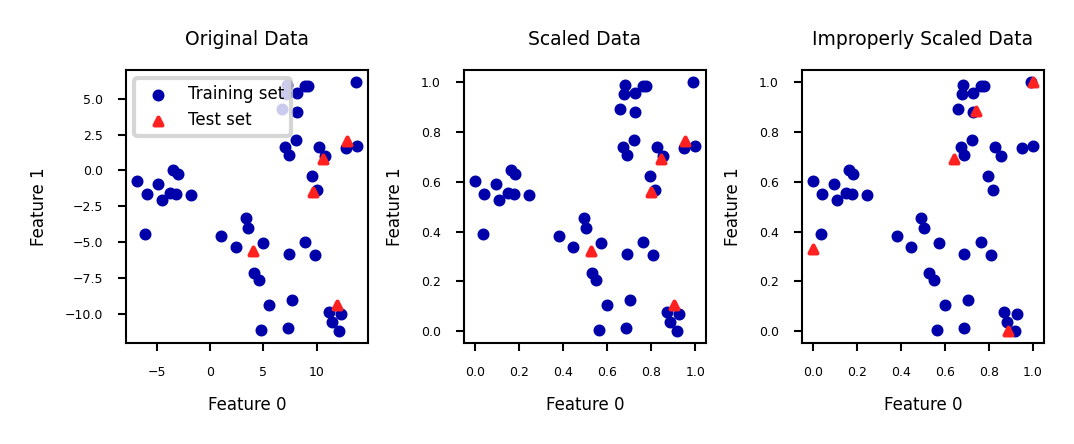
\includegraphics[width=0.9\textwidth,keepaspectratio]{images/pre-processing/distortion_1.png}
    \end{figure}
\end{frame}


